\documentclass{beamer}

\mode<presentation>

\title{Symbolic Music Similarity}
\subtitle{Presentation}
\author{Ali Bektas \and Paul Kröger}

\usepackage{graphicx}
\graphicspath{{./images/}}

\usepackage{verbatim}

%\usepackage{media9}
%\addmediapath{./audio_files/}

\usepackage{mathtools}

\usetheme{Antibes}
\setbeamertemplate{section in toc}[sections numbered]
\setbeamertemplate{subsection in toc}[subsections numbered]


\AtBeginSubsection[]
{
   \begin{frame}
        \frametitle{Inhalts\"ubersicht}
        \tableofcontents[currentsection,currentsubsection]
   \end{frame}
}

\begin{document}
	
	\begin{frame}\maketitle \end{frame}
	\begin{frame}{Überblick} \tableofcontents \end{frame}

	\section{Grundlegendes}

	\begin{frame}
  		\frametitle{Darstellung von Noten}
  		\begin{minipage}{0.45\textwidth}
  			\begin{itemize}
			\item Melodie : \textit{"singbare, in sich geschlossene Folge von Tönen"} \cite{duden_melodie}
			\item Harmonie : \textit{"wohltönender Zusammenklang mehrerer Töne oder Akkorde"} \cite{duden_harmonie}
			\item Schlüssel : \textit{"dient in der Musiknotation dazu, im Notensystem festzulegen, welche Tonhöhe die fünf Notenlinien repräsentieren."} \cite{def_schlussel}
			\end{itemize}
		\end{minipage}%
		\begin{minipage}{0.45\textwidth}
			\begin{figure}[h!]
				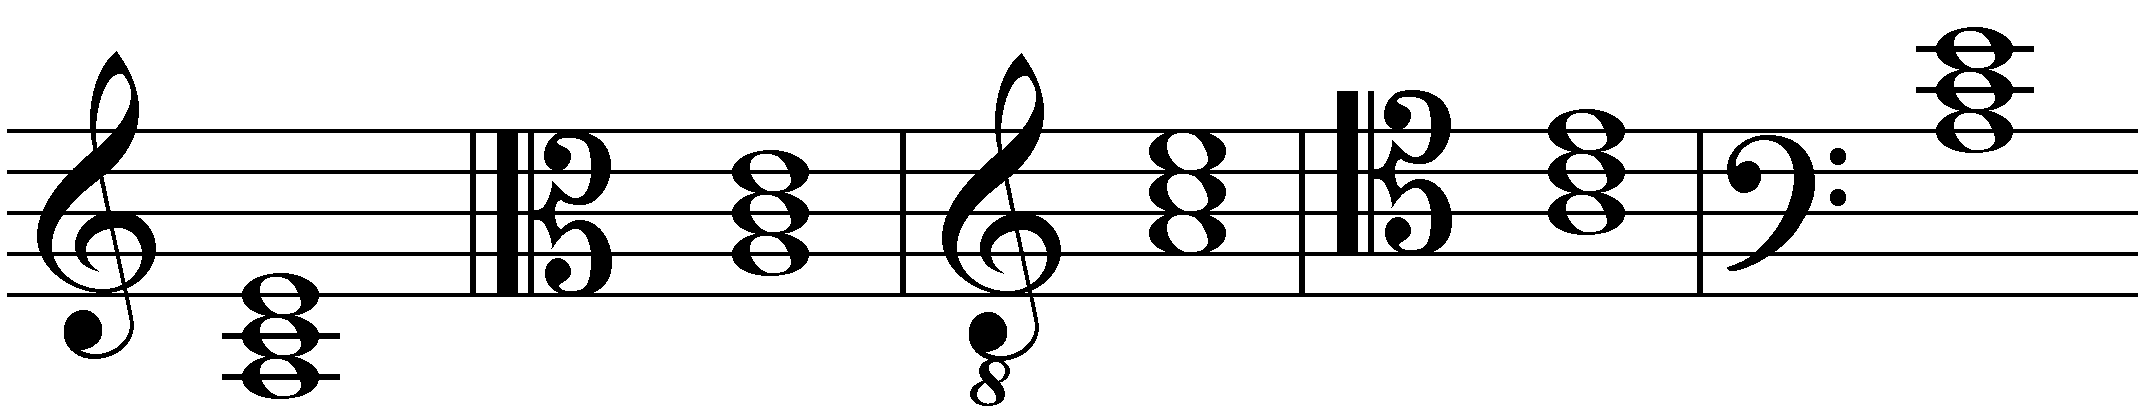
\includegraphics[width=100px,height=100px,keepaspectratio]{Clefs_chord.png}
				\caption{Source: \cite{def_schlussel}}
			\end{figure}
		\end{minipage}
	\end{frame}

	\begin{frame}
		\frametitle{Darstellung von Noten}
		Im Grunde genommen , ermöglicht die herkömmliche Methode von Notendarstellung , Informationen über Rhytmus , Tonlage , Gefühl beim Spielen , vortragsbetreffliche Elemente zu übermitteln.
		\begin{figure}[h!]
			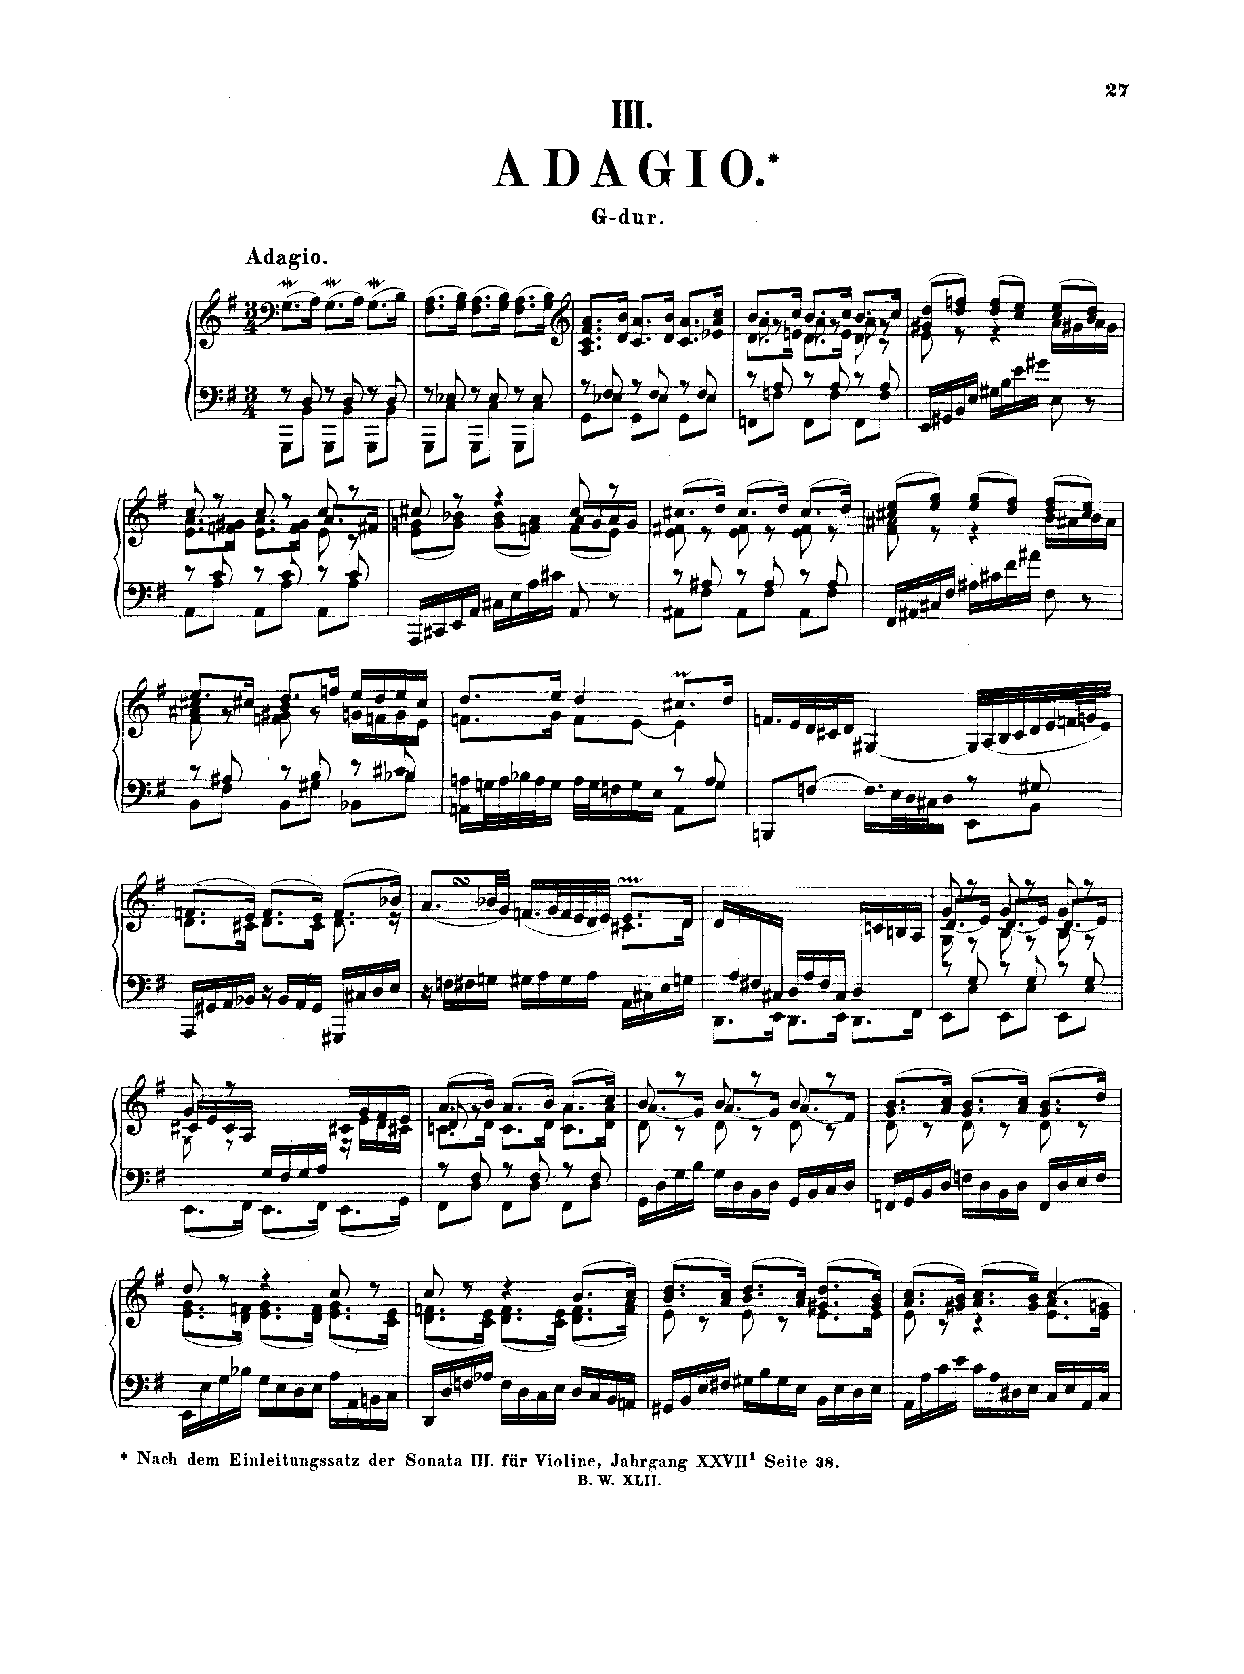
\includegraphics[width=250px,height=125px,keepaspectratio]{bach_adagio}
			\caption{Source: IMLSP Archive}
		\end{figure}
	\end{frame}

	\begin{frame}
		\frametitle{Darstellung von Noten}
			\textit{"Representing music as a weighted point set in a two-dimensional space has a tradition of many centuries. Since approximately the 10th century, one popular way of writing music has been to use a set of notes (points) in a two-dimensional space, with time and pitch as coordinates."}\cite{three}
	\end{frame}

	\section{A Section Name To Say "Different Approaches"}

	\begin{frame}
		\frametitle{Ein Graphbasierter Ansatz}
		\begin{minipage}{0.45\textwidth}
			\begin{center}
				\textit{"A Measure of Melodic Similarity Based on a Graph Representation of the Music Structure"} 
				\cite{two_point_four}  \\ 
				von Nicola Orio und Antonio Rodá.
			\end{center}
		\end{minipage}%
		\begin{minipage}{0.45\textwidth}
			\begin{figure}[h!]
				\fbox{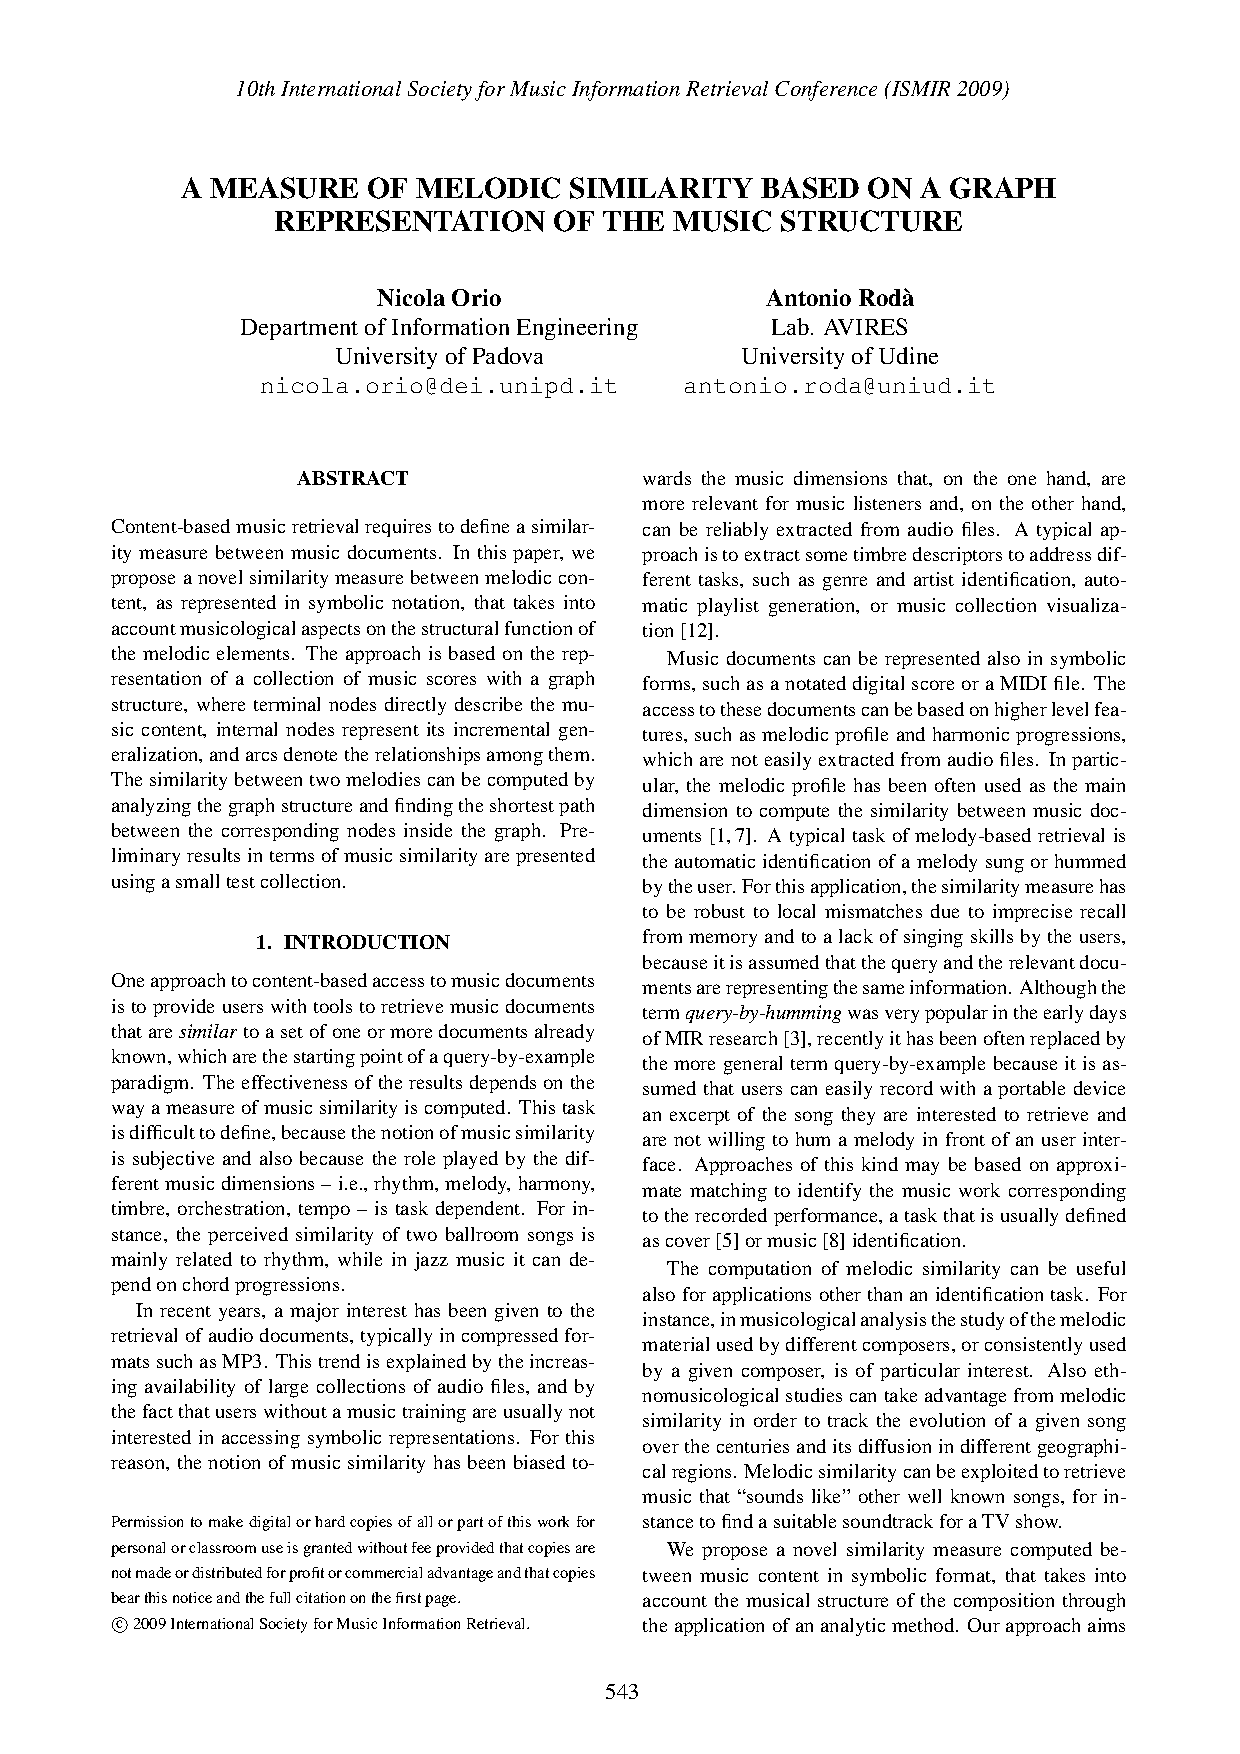
\includegraphics[width=100px,height=100px,keepaspectratio,page=1]{a_measure_of_melodic_similarity_based_on_a_graoh_representation_of_the_music_structure}}
			\end{figure}
		\end{minipage}
	\end{frame}


	\begin{frame}
		\frametitle{Ein Graphbasierter Ansatz}
		\begin{itemize}
				\item Der Inhalt wird schrittweise vereinfacht.
				\item Dazu sind die \textbf{Gewichte} der einzelnen Noten von Bedeutung.
					\begin{itemize}
						\item die unterliegende harmonische Funktion (harmonic weight)
						\item die metrische Position (metric weight)
						\item die Differenz der Tonlagen zwischen dem Ton und dem Grundton(melodic weight)
					\end{itemize}
		\end{itemize}
	\end{frame}


	\begin{frame}
		\frametitle{Ein Graphbasierter Ansatz}
		\begin{figure}[h!]
			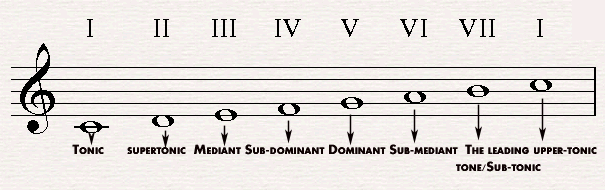
\includegraphics[width=250px,height=125px,keepaspectratio]{functional_degrees}
			\caption{Funktionen der Noten im Skala \cite{functional_degrees_source}} 
		\end{figure}
	\end{frame}


	\begin{frame}
		\frametitle{Ein auf Graphen beruhender Ansatz}
		\begin{itemize}
				\item Der Inhalt wird schrittweise vereinfacht.
				\item Dazu sind die \textbf{Gewichte} der einzelnen Noten von Bedeutung.
					\begin{itemize}
						\item die unterliegende harmonische Funktion (harmonic weight)
						\item die metrische Position (metric weight)
						\item die Differenz der Tonlagen zwischen dem Ton und dem Grundton(melodic weight)
					\end{itemize}
		\end{itemize}
	\end{frame}
	
    \begin{frame}
		\frametitle{Ein mathematischer Ansatz}
		\begin{minipage}{0.45\textwidth}
			\begin{center}
				\textit{"Algorithms for Computing Geometric Measures of Melodic Similarity"} 
				\cite{one}  \\ 
				von Greg Aloupis, Thomas Fevens, Stefan Langerman, Tomomi Matsui, Antonio Mesa, Yurai Nunez, David Rappaport, and Godfried Toussaint
			\end{center}
		\end{minipage}%
		\begin{minipage}{0.45\textwidth}
			\begin{figure}[h!]
				\fbox{\includegraphics[width=100px,height=100px,keepaspectratio,page=2]{algorithms_for_computing_geometric_measures_of_melodic_similarity}}
			\end{figure}
		\end{minipage}
	\end{frame}
	
	\begin{frame}
        \frametitle{Ein mathematischer Ansatz}
        \begin{minipage}{0.45\textwidth}
            \begin{itemize}
             \item Melodien werden als Polygonalketten dargestellt
             \item Tonlänge wird durch Länge der waagerechten Kanten modelliert
             \item Intervalle werden durch Länge der senkrechten Kanten modelliert 
            \end{itemize}
        \end{minipage}
        \begin{minipage}{0.45\textwidth}
            \fbox{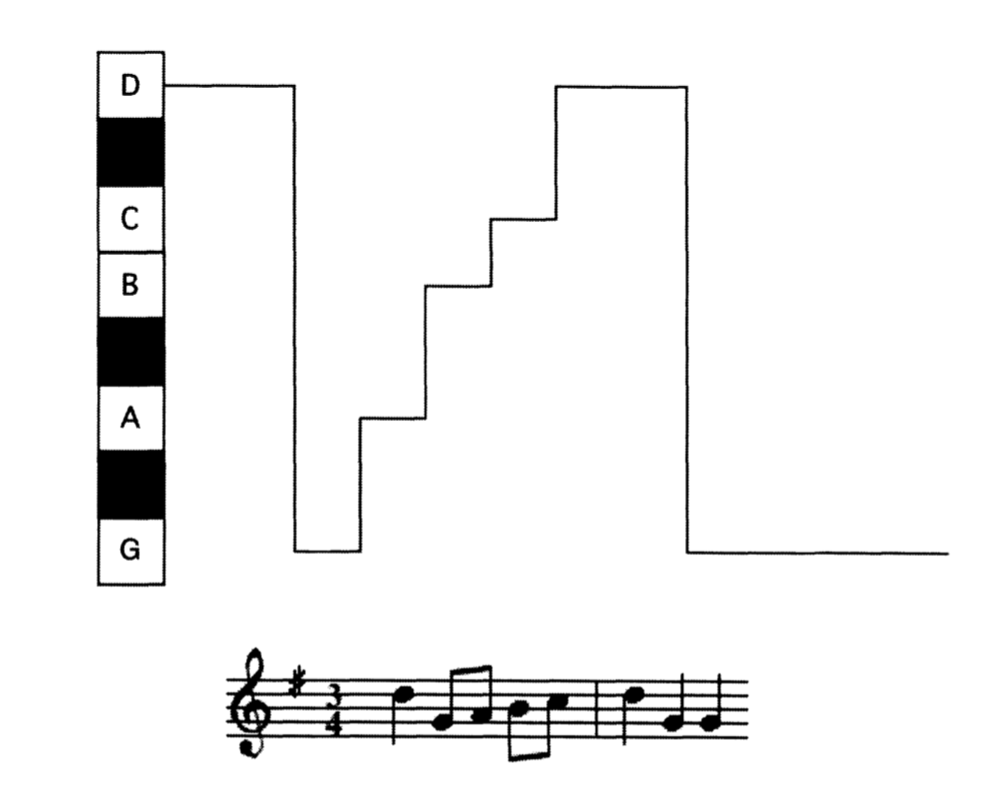
\includegraphics[width=150px,height=150px,keepaspectratio]{abb_1}}
        \end{minipage}
	\end{frame}

	\begin{frame}
        \frametitle{Insert Title}
       	\fbox{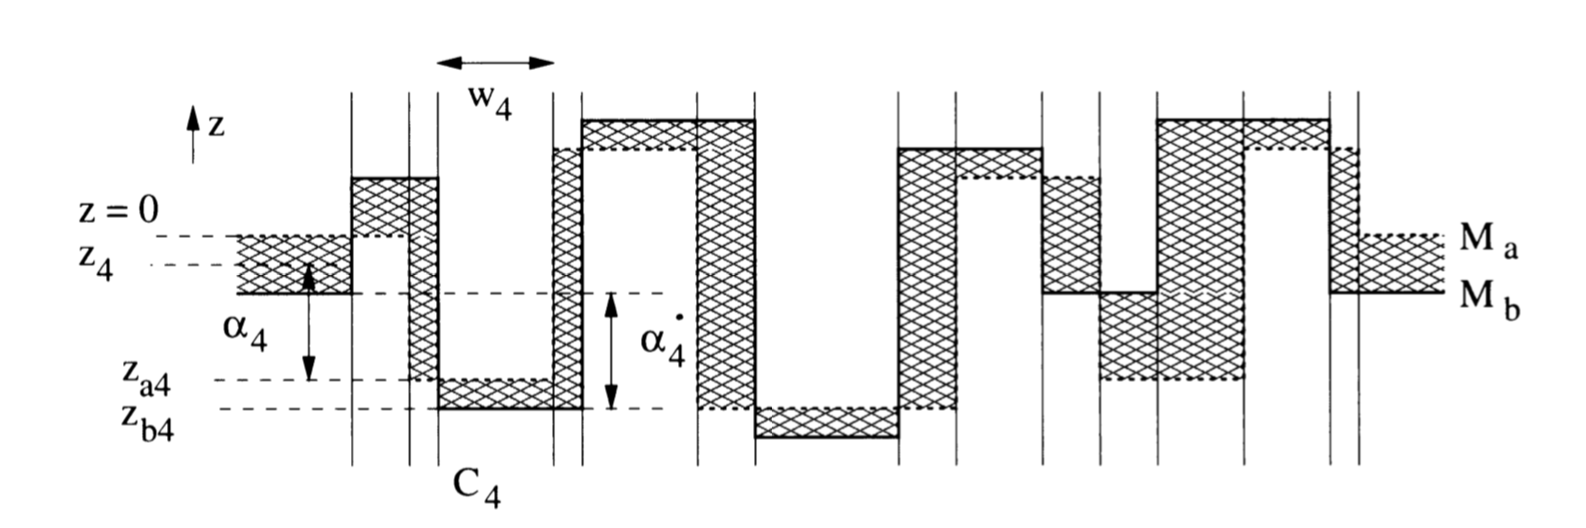
\includegraphics[width=0.7\textwidth]{abb_2}}%
        \fbox{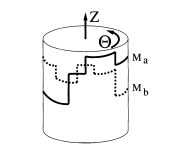
\includegraphics[width=0.3\textwidth]{abb_3}}
	\end{frame}

	\section{MIREX : Algorithmen treten gegeneinander an}

	\begin{frame}
		\frametitle{MIREX}
		\begin{itemize}
			\item Ein Wettbewerb und Plattform für Interessierte
			\item Es gibt verschiedene Kategorien
				\begin{itemize}
					\item Real-time Audio to Score Alignment (a.k.a Score Following)
					\item Discovery of Repeated Themes and Sections
					\item Audio Melody Extraction
					\item \textbf{Symbolic Melodic Similarity}
					\item ...
				\end{itemize}
			\item Gegeben ein Ziel , treten verschiedene Algorithmen gegeneinander zum Wettkampf an. Derjenige, der die besten Ergebnisse hat , gewinnt. 
			\item \textbf{Nun eine Frage:}Wie kann man Algorithmen miteinander vergleichen?
			\item Es kommt nicht auf die Laufzeit oder Speicherbedarf an , sondern auf die Qualität der Ergebnisse.
			\item Welche Messmethoden gibt es , um die Qualität von solcen Ergebnissen zu beurteilen?
		\end{itemize}
	\end{frame}

	\begin{frame}
		\frametitle{MIREX}
		\begin{figure}[h!]
			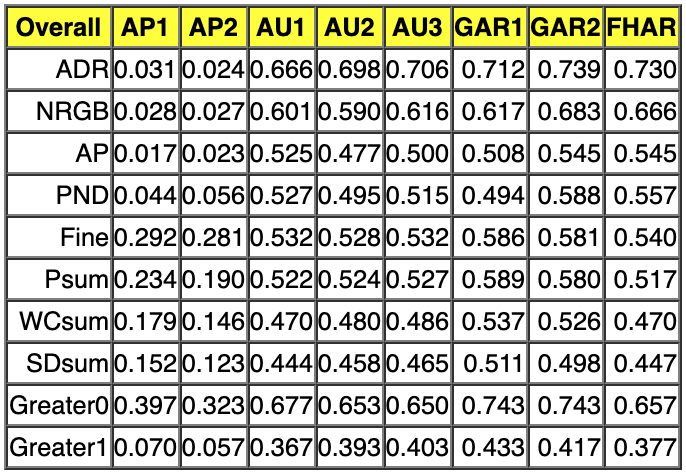
\includegraphics[width=300px,height=150px,keepaspectratio]{mirex_result_example}
			\caption{Source: \cite{mirex_website_2007_results}}
		\end{figure}
	\end{frame}


	\begin{frame}
		\frametitle{MIREX}
		\begin{figure}[h!]
			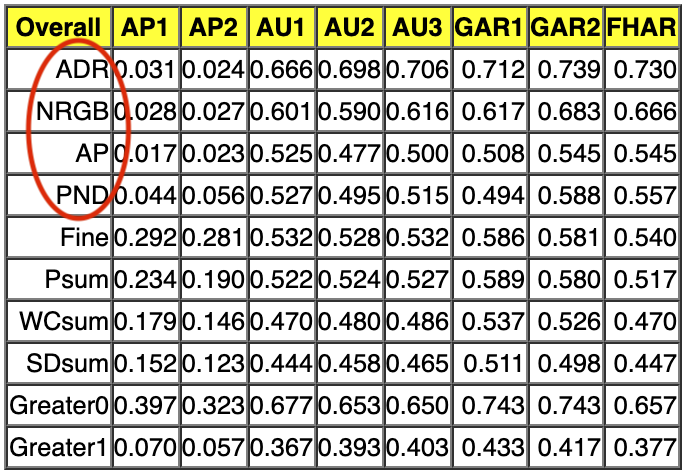
\includegraphics[width=300px,height=150px,keepaspectratio]{mirex_result_example_change_one}
		\end{figure}
	\end{frame}

	\subsection{Ground Truth}
		
		\begin{frame}
			\frametitle{Ground Truth}
			\begin{itemize}
				\item Experten werden befragt , Stücke aus der RISM A/II Sammlung  nach deren Ähnlichkeiten zu einer Anfrage zu beurteilen.
				\item Die Sammlungen sind groß deswegen sind einige Techniken zur Eliminierung unrelevanter Elementen vorzunehmen , wie z.B
					\begin{itemize}
						\item Nach der Differenz zwischen dem tiefsten und höchsten Ton.
						\item Nach dem Verhältnis der kürzesten Note zu der längsten.
						\item usw.
					\end{itemize}
				\item Nicht für alle Stücke werden dieselben Elimierungsverfahren vorgenommen. Die Aspekte , durch die sich ein Stück auszeichnet sind beizubehalten. Das ist wiederum für die Experten zu entscheiden.
			\end{itemize}
		\end{frame}

		\begin{frame}[allowframebreaks]
			\frametitle{Ground Truth}
				\begin{figure}[h!]
					
\includegraphics[width=300px,height=75px,keepaspectratio]{ground_truth_query}
					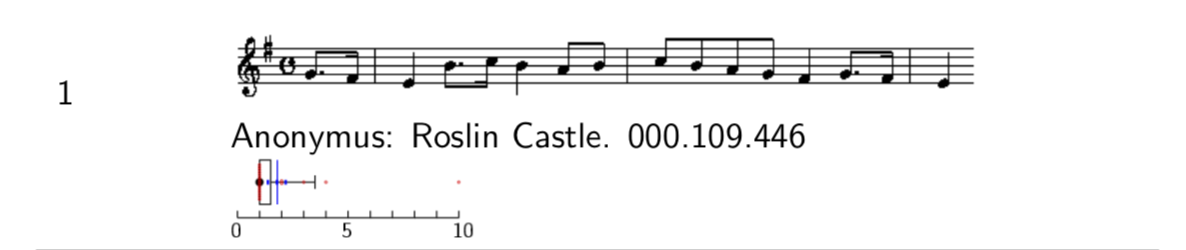
\includegraphics[width=300px,height=75px,keepaspectratio]{ground_truth_results_one}
					\caption{Abbildung: Ergebnisse der Befragung \cite{three}}
				\end{figure}
				\begin{figure}[h!]
					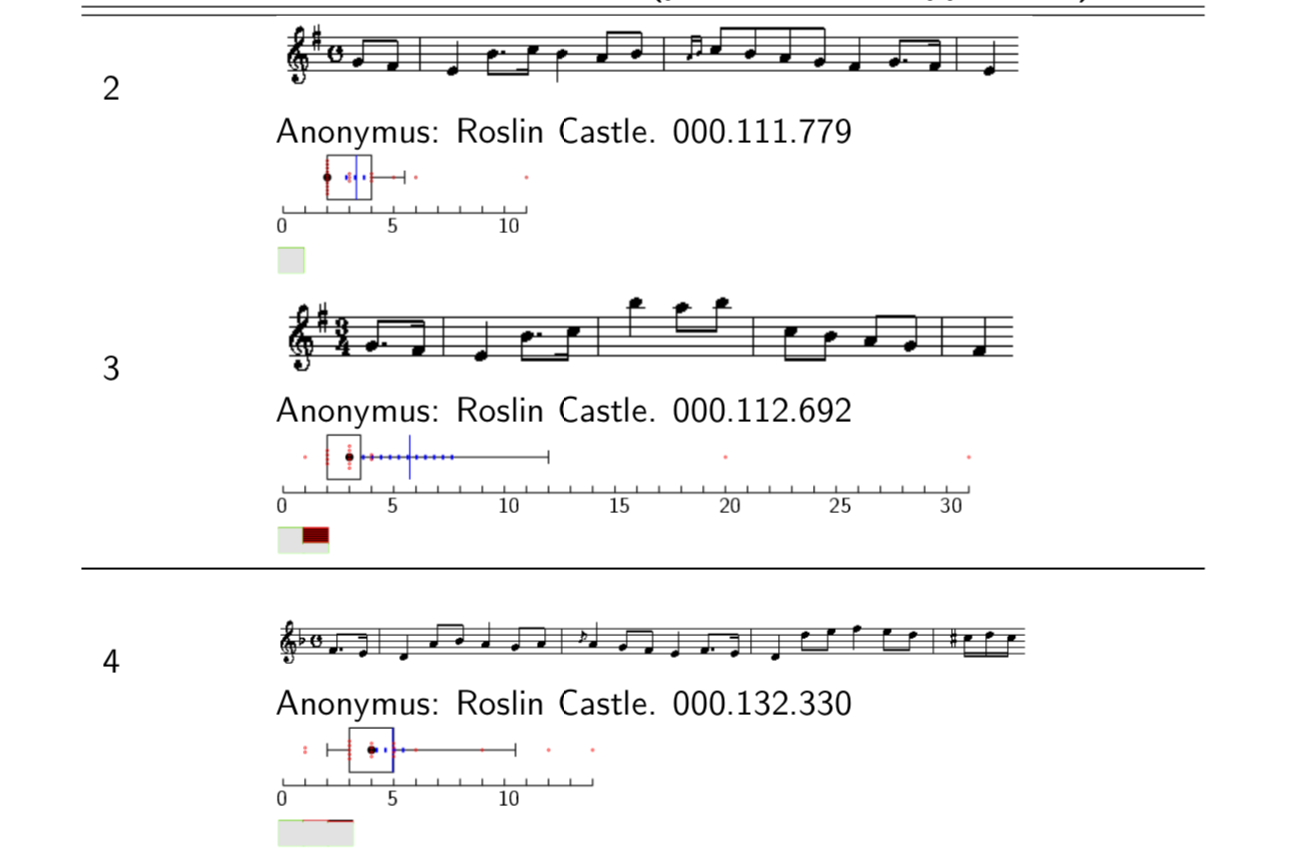
\includegraphics[width=300px,height=150px,keepaspectratio]{ground_truth_results_two}
				\end{figure}
				\begin{figure}[h!]
					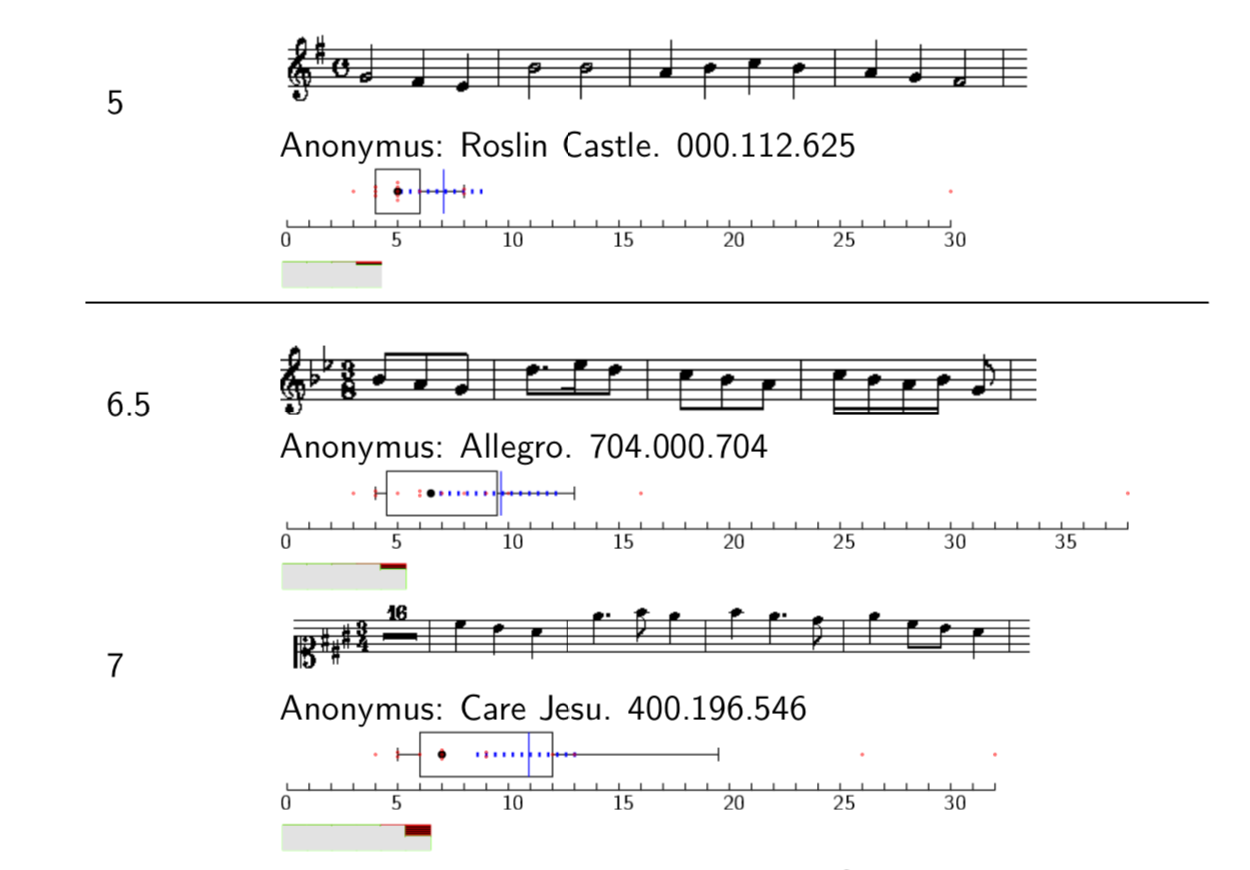
\includegraphics[width=300px,height=150px,keepaspectratio]{ground_truth_results_three}
				\end{figure}
		\end{frame}

	\begin{frame}
		\frametitle{MIREX}
		\begin{figure}[h!]
			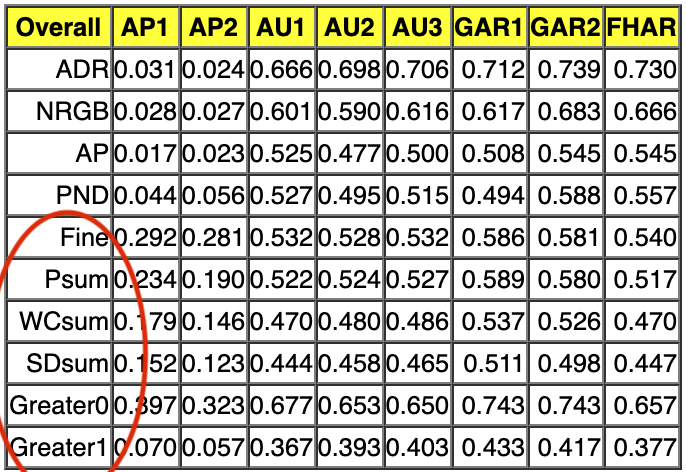
\includegraphics[width=300px,height=150px,keepaspectratio]{mirex_result_example_change_two}
		\end{figure}
	\end{frame}

	\subsection{Average Dynamic Recall}

		\begin{frame}
			\frametitle{Beispiel : Average Dynamic Recall - ADR}
			\begin{figure}[h!]
				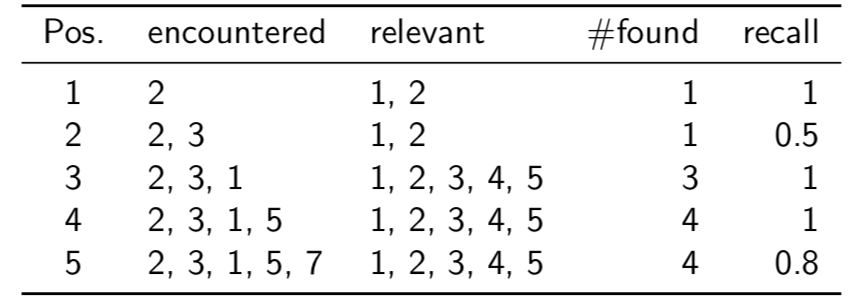
\includegraphics[width=300px,height=150px,keepaspectratio]{adr_example}
				\caption{Abbildung: ADR Berechnung \cite{three}}
			\end{figure}
		\end{frame}

	\subsection{MIREX 2005}
		\begin{frame}
			\frametitle{MIREX 2005}
			\begin{minipage}{0.45\textwidth}
				\begin{center}
					\textit{"Melody Retrieval using the Implication/Realization Model"} 
					\cite{mirex_2005_one}\\ 
					Maarten Grachten, Josep Lluis Arcos and Ramon Lopez de Mantaras 
				\end{center}
			\end{minipage}%
			\begin{minipage}{0.45\textwidth}
				\begin{figure}[h!]
					\fbox{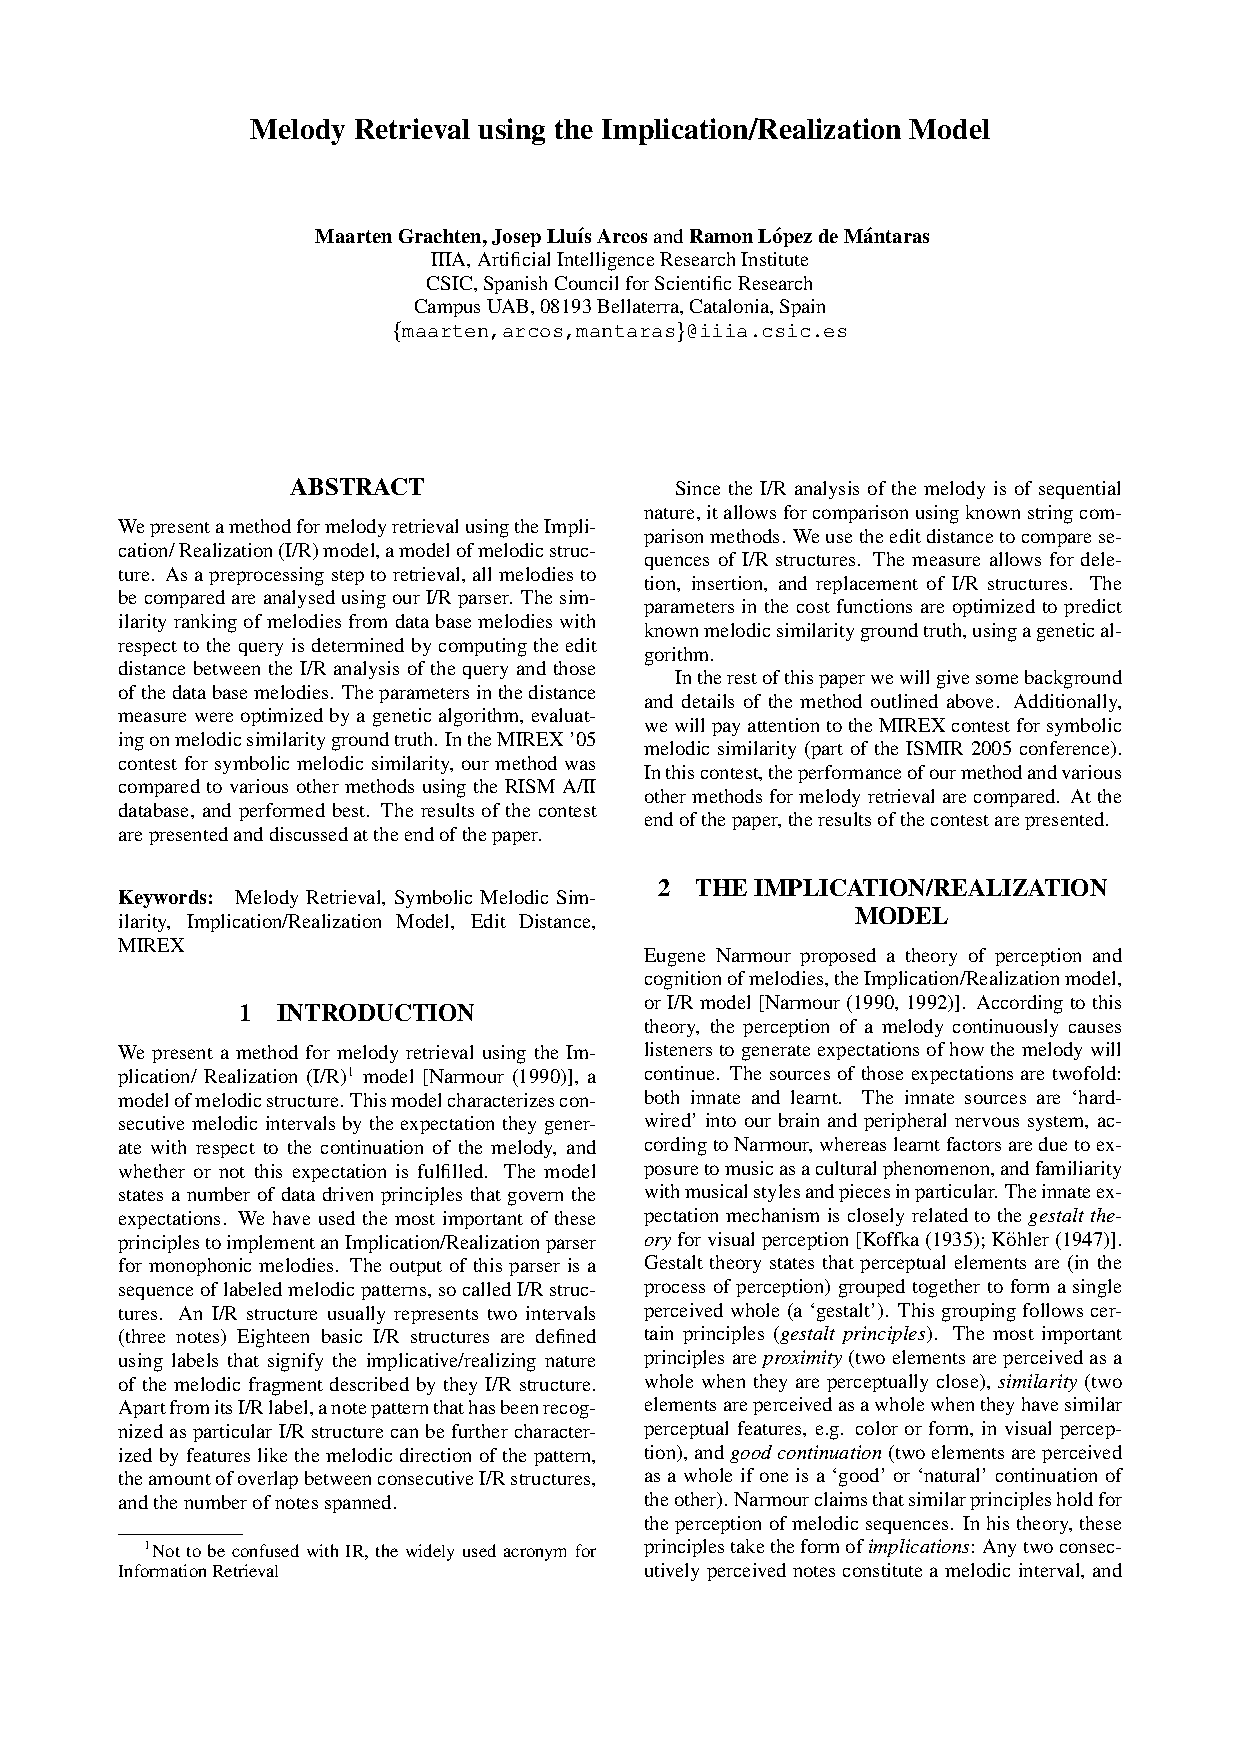
\includegraphics[width=100px,height=100px,keepaspectratio,page=1]{mirex_2005_one.pdf}}
				\end{figure}
			\end{minipage}
		\end{frame}

		\begin{frame}
			\frametitle{MIREX 2005}
			
			\begin{itemize}
				\item Ein auf Kognitivwissenschaften basierendes Modell : Implication/Realization Model.
				\item Dies besagt , dass man nach seinen Erfahrungen (sowohl kulturellen , als auch angeborenen) Erwartungen hat , wie ein Musikstück weitergeht. 
				\item Wir beschäftigen uns hier mit den angeborenen Aspekten.
				\item I/R Modell besagt : Wir sind dazu geneigt , Elemente nach Konzepten zu gruppieren. Diese Konzepten sind denen der Gestalttheorie ähnlich
					\begin{itemize}
						\item Proximity : Werden zwei Elemente gleich wahrgenommen?
						\item Similarity : Haben zwei Elemente Ähnlichkeiten?
					\end{itemize}
			\end{itemize}
		\end{frame}


		\begin{frame}
			\frametitle{MIREX 2005}
			\begin{itemize}
				\item PRD : kleines Intervall in eine Richtung impliziert noch ein Intervall in dieselbe Richtung
				\item PID : kleines Intervall impliziert ein kleines Intervall.
				\item Nach diesen Prinzipien ist ein Alphabet von Strukturen definiert.
				\item Mithilfe von Edit Distance wird die Ähnlichkeit festgestellt.
			\end{itemize}
		\end{frame}


		\begin{frame}[allowframebreaks]
			\frametitle{MIREX 2005}
			\begin{figure}[h!]
					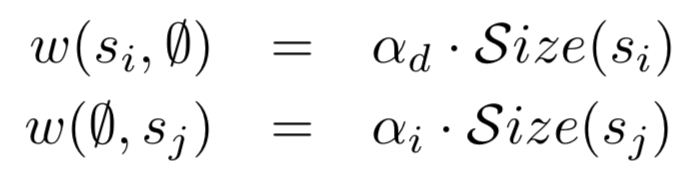
\includegraphics[width=300px,height=30px,keepaspectratio]{mirex_2005_one_img_one}
			\end{figure}
			\begin{figure}[h!]
					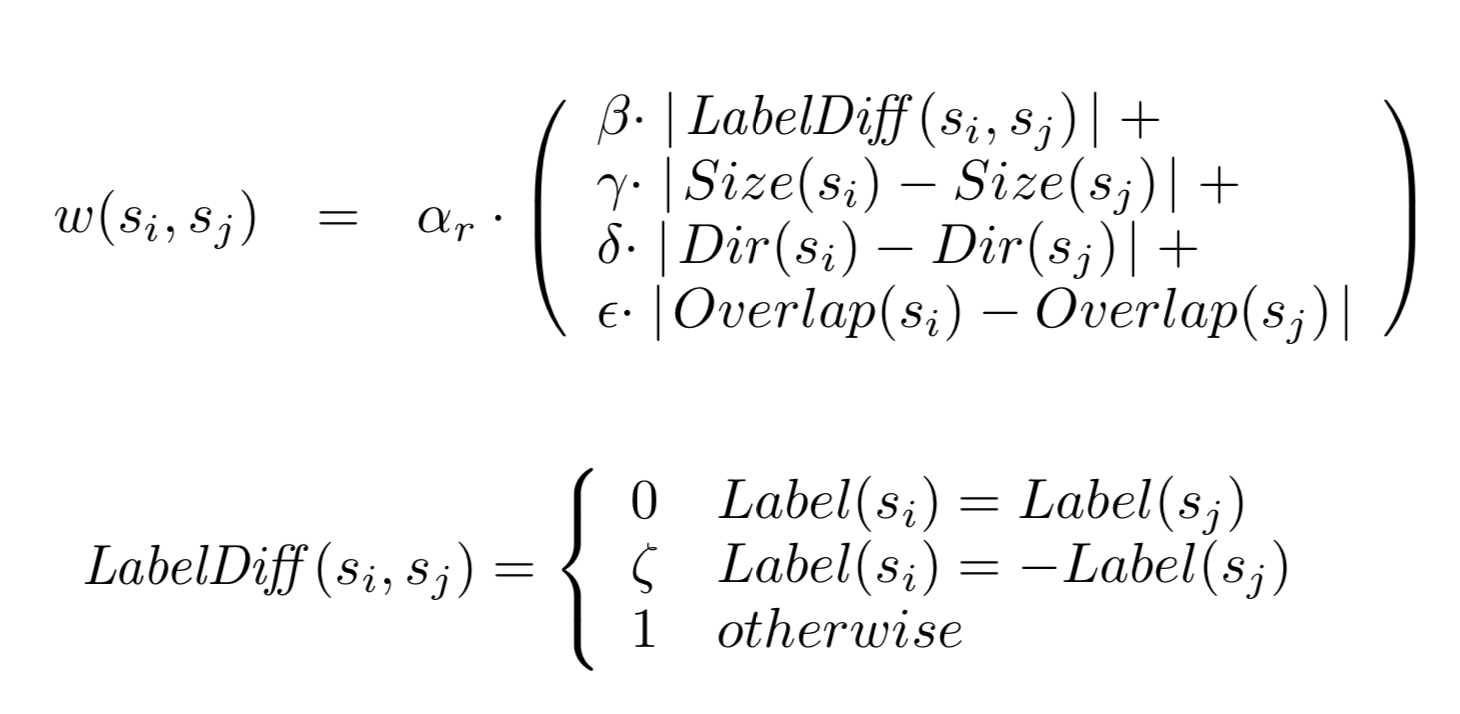
\includegraphics[width=300px,height=150px,keepaspectratio]{mirex_2005_one_img_two}
			\end{figure}
			\begin{figure}[h!]
					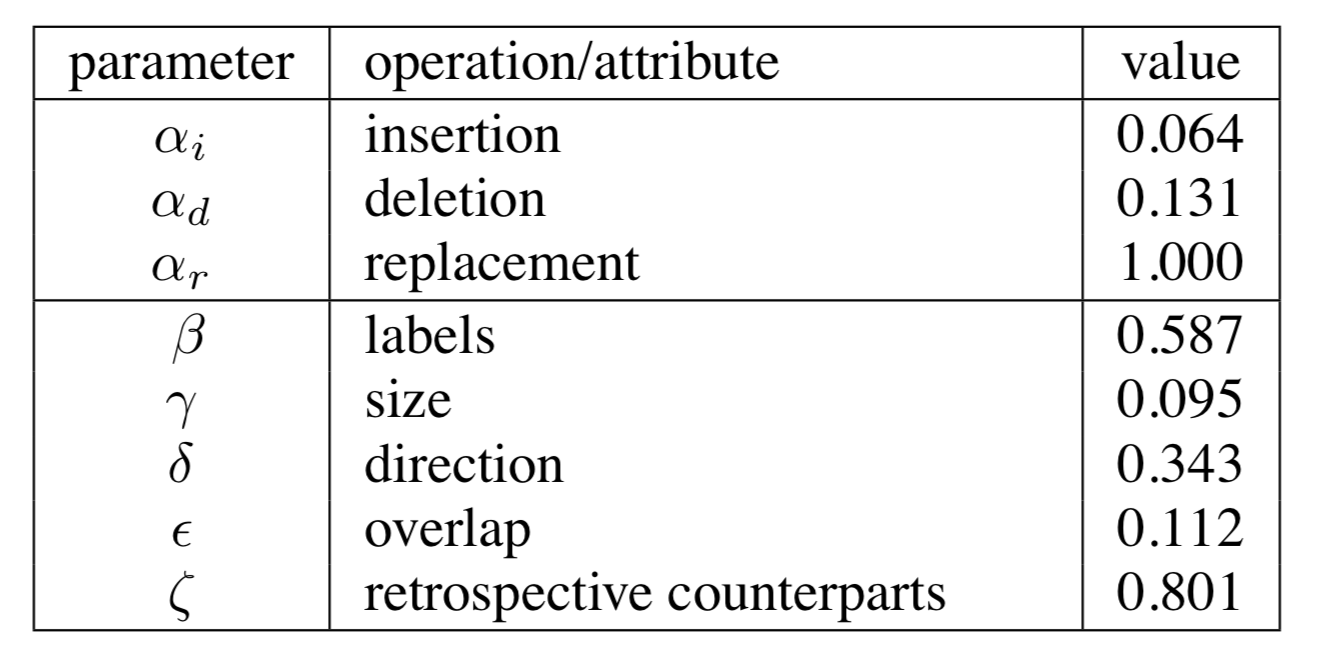
\includegraphics[width=300px,height=150px,keepaspectratio]{mirex_2005_one_img_three}
			\end{figure}
		\end{frame}


		\begin{frame}
			\frametitle{MIREX 2005}
			\begin{minipage}{0.45\textwidth}
				\begin{center}
					\textit{"Combining Multilevel and Multifeature Representation to Compute Melodic Similarity"} 
					\cite{mirex_2005_two}\\ 
					Nicola Orio
				\end{center}
			\end{minipage}%
			\begin{minipage}{0.45\textwidth}
				\begin{figure}[h!]
					\fbox{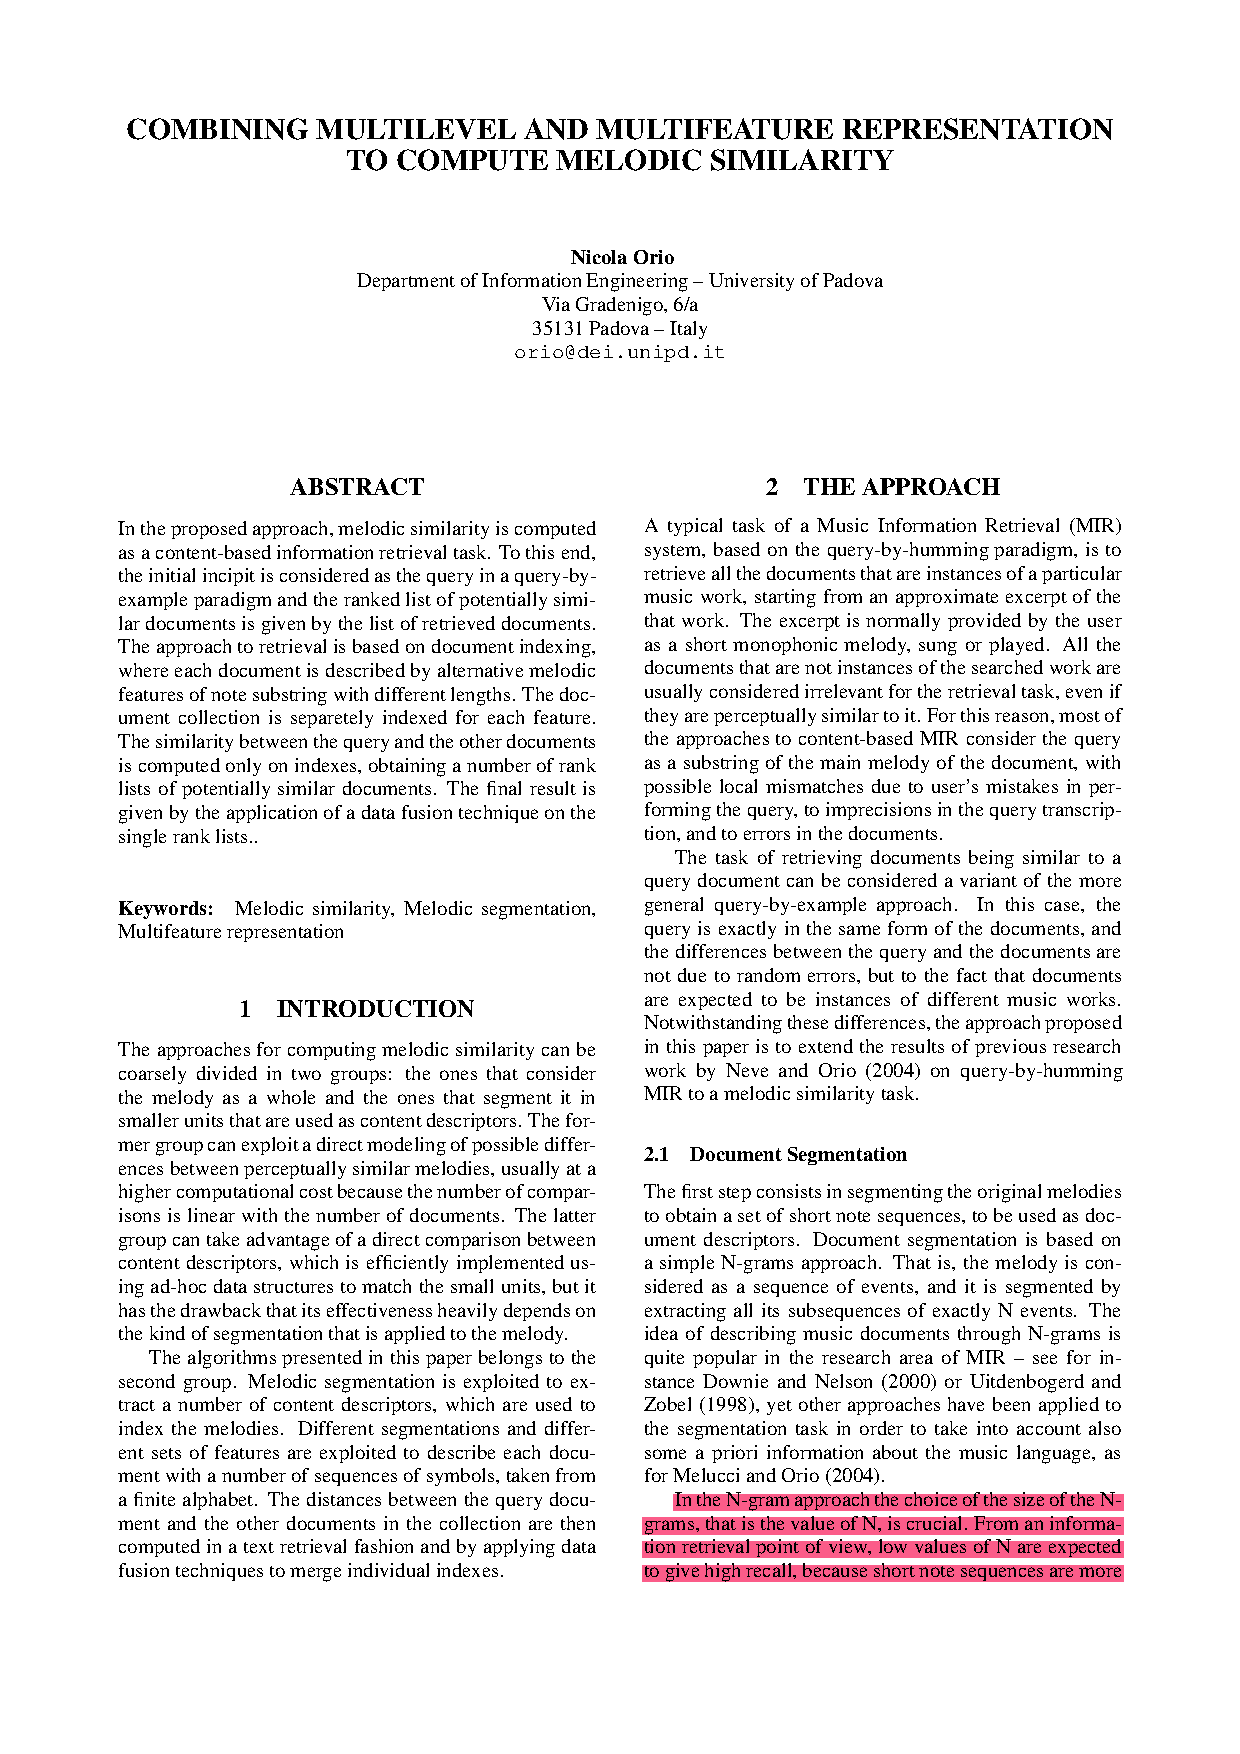
\includegraphics[width=100px,height=100px,keepaspectratio,page=1]{mirex_2005_two.pdf}}
				\end{figure}
			\end{minipage}
		\end{frame}

		\begin{frame}
			\begin{itemize}
				\item N-gram 
				\item Jede Wahl von N hat Vor- und Nachteile. Um diese zu beseitigen wird Multilevel Segmentation eingesetzt.
			\end{itemize}
		\end{frame}

		\begin{frame}
			\begin{figure}[h!]
				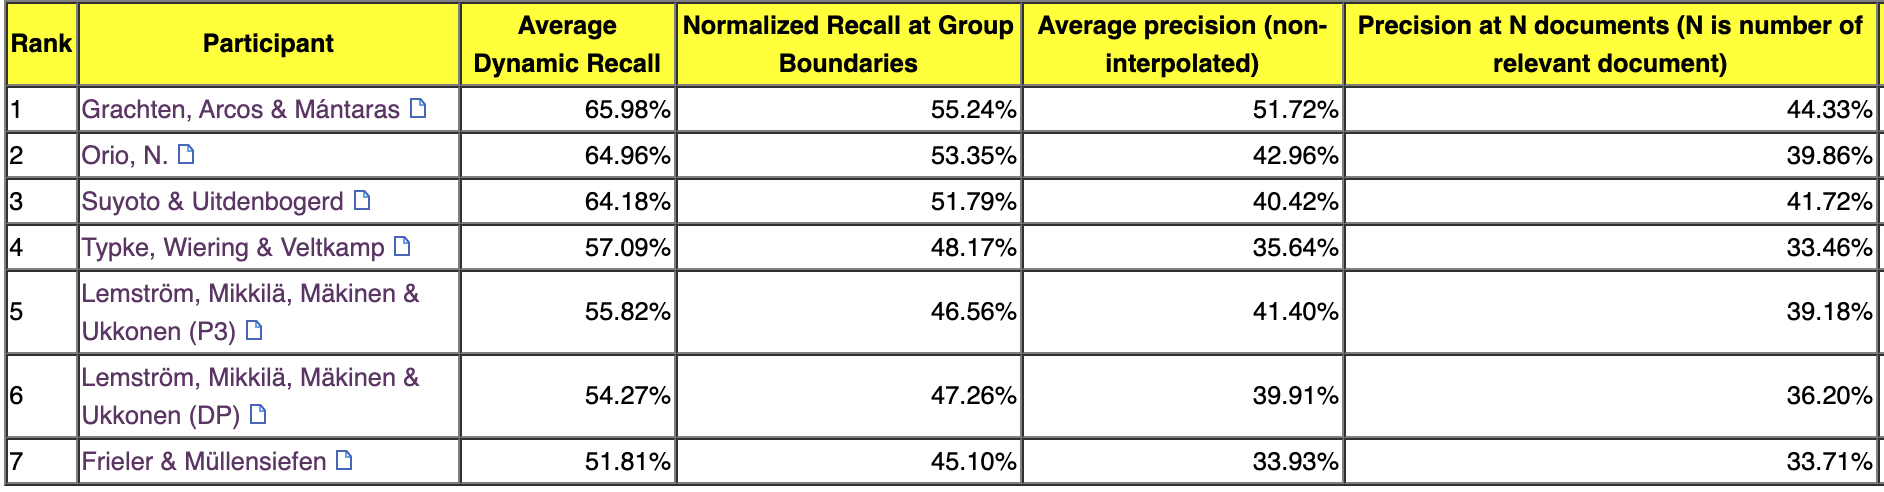
\includegraphics[width=300px,height=30px,keepaspectratio]{mirex_2005_results}
			\end{figure}
		\end{frame}

	
	
	\subsection{Urbano MelodyShape}
		\begin{frame}
			\frametitle{Urbano MelodyShap}
			\begin{minipage}{0.45\textwidth}
				\begin{center}
					\textit{"MelodyShape at MIREX 2014 Symbolic Melodic Similarity"} 
					\cite{five_point_two}\\ 
					von Julian Urbano
				\end{center}
			\end{minipage}%
			\begin{minipage}{0.45\textwidth}
				\begin{figure}[h!]
					\fbox{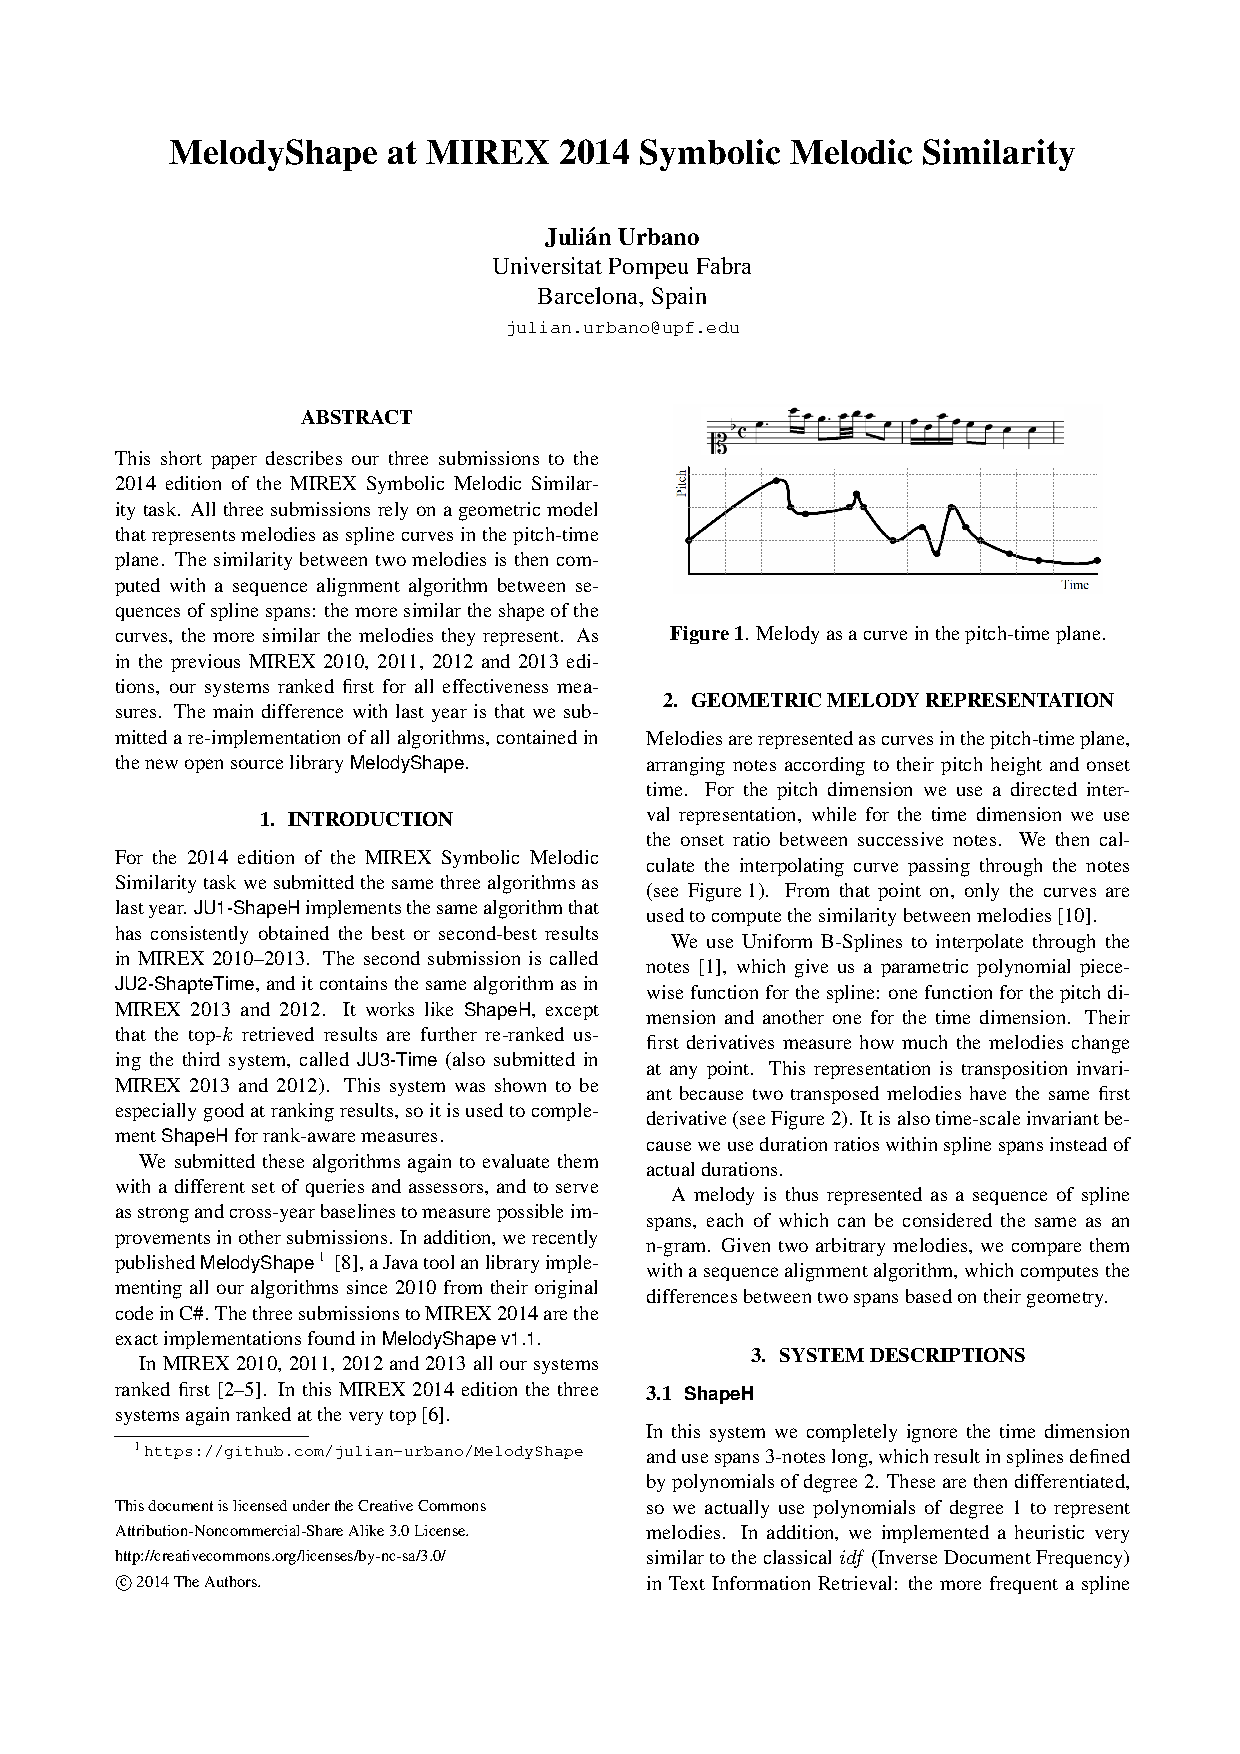
\includegraphics[width=100px,height=100px,keepaspectratio,page=1]{JU1}}
				\end{figure}
			\end{minipage}
		\end{frame}
		
	\begin{frame}
        \frametitle{Urbano MelodyShape}
        \begin{minipage}{0.45\textwidth}
            \begin{itemize}
             \item Töne werden als Punkt  auf Pitch-Time plane dargestellt.
             \item Darstellung als Funktion durch Interpolation mithile von Splines.
            \end{itemize}
        \end{minipage}
        \begin{minipage}{0.45\textwidth}
            \fbox{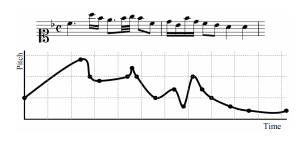
\includegraphics[width=150px,height=150px,keepaspectratio]{abb_4}}
        \end{minipage}
	\end{frame}
	
    \begin{frame}
        \frametitle{Needlemann - Wunsch Algorithmus}
       \fbox{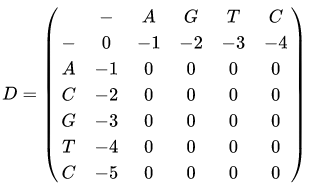
\includegraphics[width=0.5\textwidth]{abb_7}}%
        \fbox{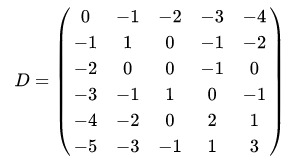
\includegraphics[width=0.5\textwidth]{abb_8}}
	\end{frame}
	
	\begin{frame}
        \frametitle{ShapeH}
        \begin{minipage}{0.45\textwidth}
            \begin{itemize}
             \item Insertion : $ s(-, n) = -(1 - f(n))$
             \item Deletion: $s(n, -) = -(1 - f(n))$
             \item Match: $s(n, n) = 1 - f(n)$
     %        \item Sequence Alignment $H(i,j) = max \{H(i - 1, j - 1) + s(a_i,b_j) \n
        %     H(i - 1, j) + s(a_i, -) \n H(i, j - 1) + s(i, b_j) \}$
            \end{itemize}
        \end{minipage}
        \begin{minipage}{0.45\textwidth}
            \fbox{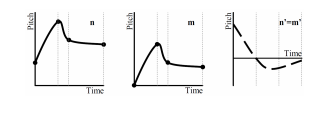
\includegraphics[width=150px,height=150px,keepaspectratio]{abb_5}}
        \end{minipage}
	\end{frame}
	
	\begin{frame}
        \frametitle{Time}
            \begin{itemize}
             \item Insertion : $ s(-, n) = -diff_p(n,\Theta (n)) - \lambda k_t * diff_t(n,\Theta (n))$
             \item Deletion: $s(n, -) = -diff_p(n,\Theta (n)) - \lambda k_t * diff_t(n,\Theta (n))$
             \item Match: $2\mu_p + 2\lambda k_t\mu_t = 2\mu_p(1+k_t)$
             \item Substitution $s(n,m) = -diff_p(n,m) - \lambda k_t * diff_t(n,m)$
            \end{itemize}
            \begin{center}
            \fbox{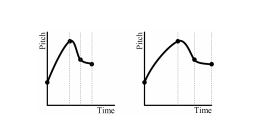
\includegraphics[width=150px,height=150px,keepaspectratio]{abb_6}}
            \end{center}
	\end{frame}
	


	\section{Bibliographie}

	\begin{frame}[allowframebreaks]
		\frametitle{Bibliographie}
		\begin{thebibliography}{5}
			\setbeamertemplate{bibliography item}[text]
			\bibitem[1]{duden_melodie} Duden: Melodie: Rechtschreibung, Bedeutung, Definition, Herkunft
			https://www.duden.de/rechtschreibung/Melodie.
			\bibitem[2]{duden_harmonie} Duden: Harmonie : Rechtschreibung, Bedeutung, Definition, Herkunft
			https://www.duden.de/rechtschreibung/Harmonie.
			\bibitem[3]{def_schlussel} “Notenschlüssel.” Wikipedia, Wikimedia Foundation, 11 Dec. 2019, de.wikipedia.org/wiki/Notenschlüssel.
			\bibitem[4]{mirex_website} MIREX,Symbolic Melodic Similarity 2005,https://www.music-ir.org/mirex/wiki/2005:Symbolic\_Melodic.
			\bibitem[5]{mirex_website_2007_results} MIREX,Symbolic Melodic Similarity Results 2007, https://www.music-ir.org/mirex/wiki/2007:Symbolic\_Melodic\_Similarity\_Results.
			\bibitem[6]{three} Typke, Rainer. (2007). Music Retrieval based on Melodic Similarity.
			\bibitem[7]{two_point_four} Orio, N., and A. Rodá. 2009. “A Measure of Melodic Similarity Based on a Graph Representation of the Music Structure.” In Proceedings of the International Conference for Music Information Retrieval, pp. 543– 548.
			\bibitem[8]{one} Greg Aloupis, Thomas Fevens, Stefan Langerman, Tomomi Matsui, Antonio Mesa, Yurai Nunez, David Rappaport, and Godfried Toussaint, "Algorithms for Computing Geometric Measures of Melodic Similarity" Computer Music Journal, Vol.30, No. 3 (Autumn, 2006), pp. 67-76
			\bibitem[9]{functional_degrees_source} Tonal Degrees [Online]. [Accessed 30 Jan 2020]. Available from : http://www.piano-play-it.com/musical-scales.html
			\bibitem[10]{five_point_two} J. Urbano. MelodyShape at MIREX 2014 Symbolic
            Melodic Similarity. Technical report, Music Information Retrieval Evaluation eXchange, 2014
            \bibitem[11]{mirex_2005_one} Grachten, Maarten \& Arcos, Josep Lluís \& Mántaras, Ramon. (2020). Melody Retrieval using the Implication/Realization Model. 
           	\bibitem[12]{mirex_2005_two} Orio, Nicola. “Combining Multilevel and Multifeature Representation to Compute Melodic Similarity.” (2005).
		\end{thebibliography}
	\end{frame}
\end{document}
